\documentclass[aps,prx,10pt,twocolumn,floatfix,superscriptaddress,showpacs,numerical,footinbib]{revtex4-1}

\usepackage{graphicx}
\usepackage{amsmath}
\usepackage{amssymb}
\usepackage[T1]{fontenc}
\usepackage[utf8]{inputenc}
\usepackage{hyperref}
\usepackage[pdftex]{color}

\newcommand{\sgn}[1]{\mathrm{sgn} \left( #1 \right)}
\newcommand{\e}{\mathrm{e}}
\newcommand{\im}{\mathrm{i}}
\newcommand{\di}{\mathrm{d}}
\newcommand{\ket}[1]{| #1 \rangle}
\newcommand{\bra}[1]{\langle #1 |}
%\renewcommand{\thefootnote}{\fnsymbol{footnote}}

\newcommand{\noteAG}[1]{{\color{blue} [AG: #1]}}
\newcommand{\noteFP}[1]{{\color{magenta} [FP: #1]}}
\newcommand{\noteJM}[1]{{\color{red} [JM: #1]}}
\newcommand{\noteFdJ}[1]{{\color{cyan} [FdJ: #1]}}
\newcommand{\bs}[1]{{\boldsymbol{#1}}}


\begin{document}
%
\title{Interaction driven phases in the half-filled honeycomb lattice: an infinite density matrix renormalization group study}
%
\author{Good people}
\affiliation{\mbox{Max-Planck-Institut f\"ur Physik komplexer Systeme, N\"othnitzer Str.\ 38, 01187 Dresden, Germany}}
%
\date{\today}
%
\begin{abstract}
%
This is an abstract.
%
\noteAG{There are specific commands to leave comments like this one}\noteFP{or this}\noteJM{or this}\noteFdJ{or this}
%
\end{abstract}
%
\maketitle
%

\section{Introduction}
%
Topological phases of matter are remarkably robust states; their responses to external fields are
governed by topological invariants and thus many of their most important properties are insensitive to local perturbations.
%
Topologically protected responses result in intrinsically novel phenomena that can find no straight forward analogue in trivial states
of matter, including frationalisation of quantum numbers or transport governed by quantum anomalies.
%
These exotic properties have inspired proposals of diverse prospective applications, ranging from quantum computation to spintronics.
%
Added to the remarkable experimental discoveries of new topological phases in both two and three dimensions,
these ideas have boosted a sustained and voluminous scientific effort in the last decade that attempts to classify them and determine when and how can they emerge.
%


%
\begin{figure}[b]
 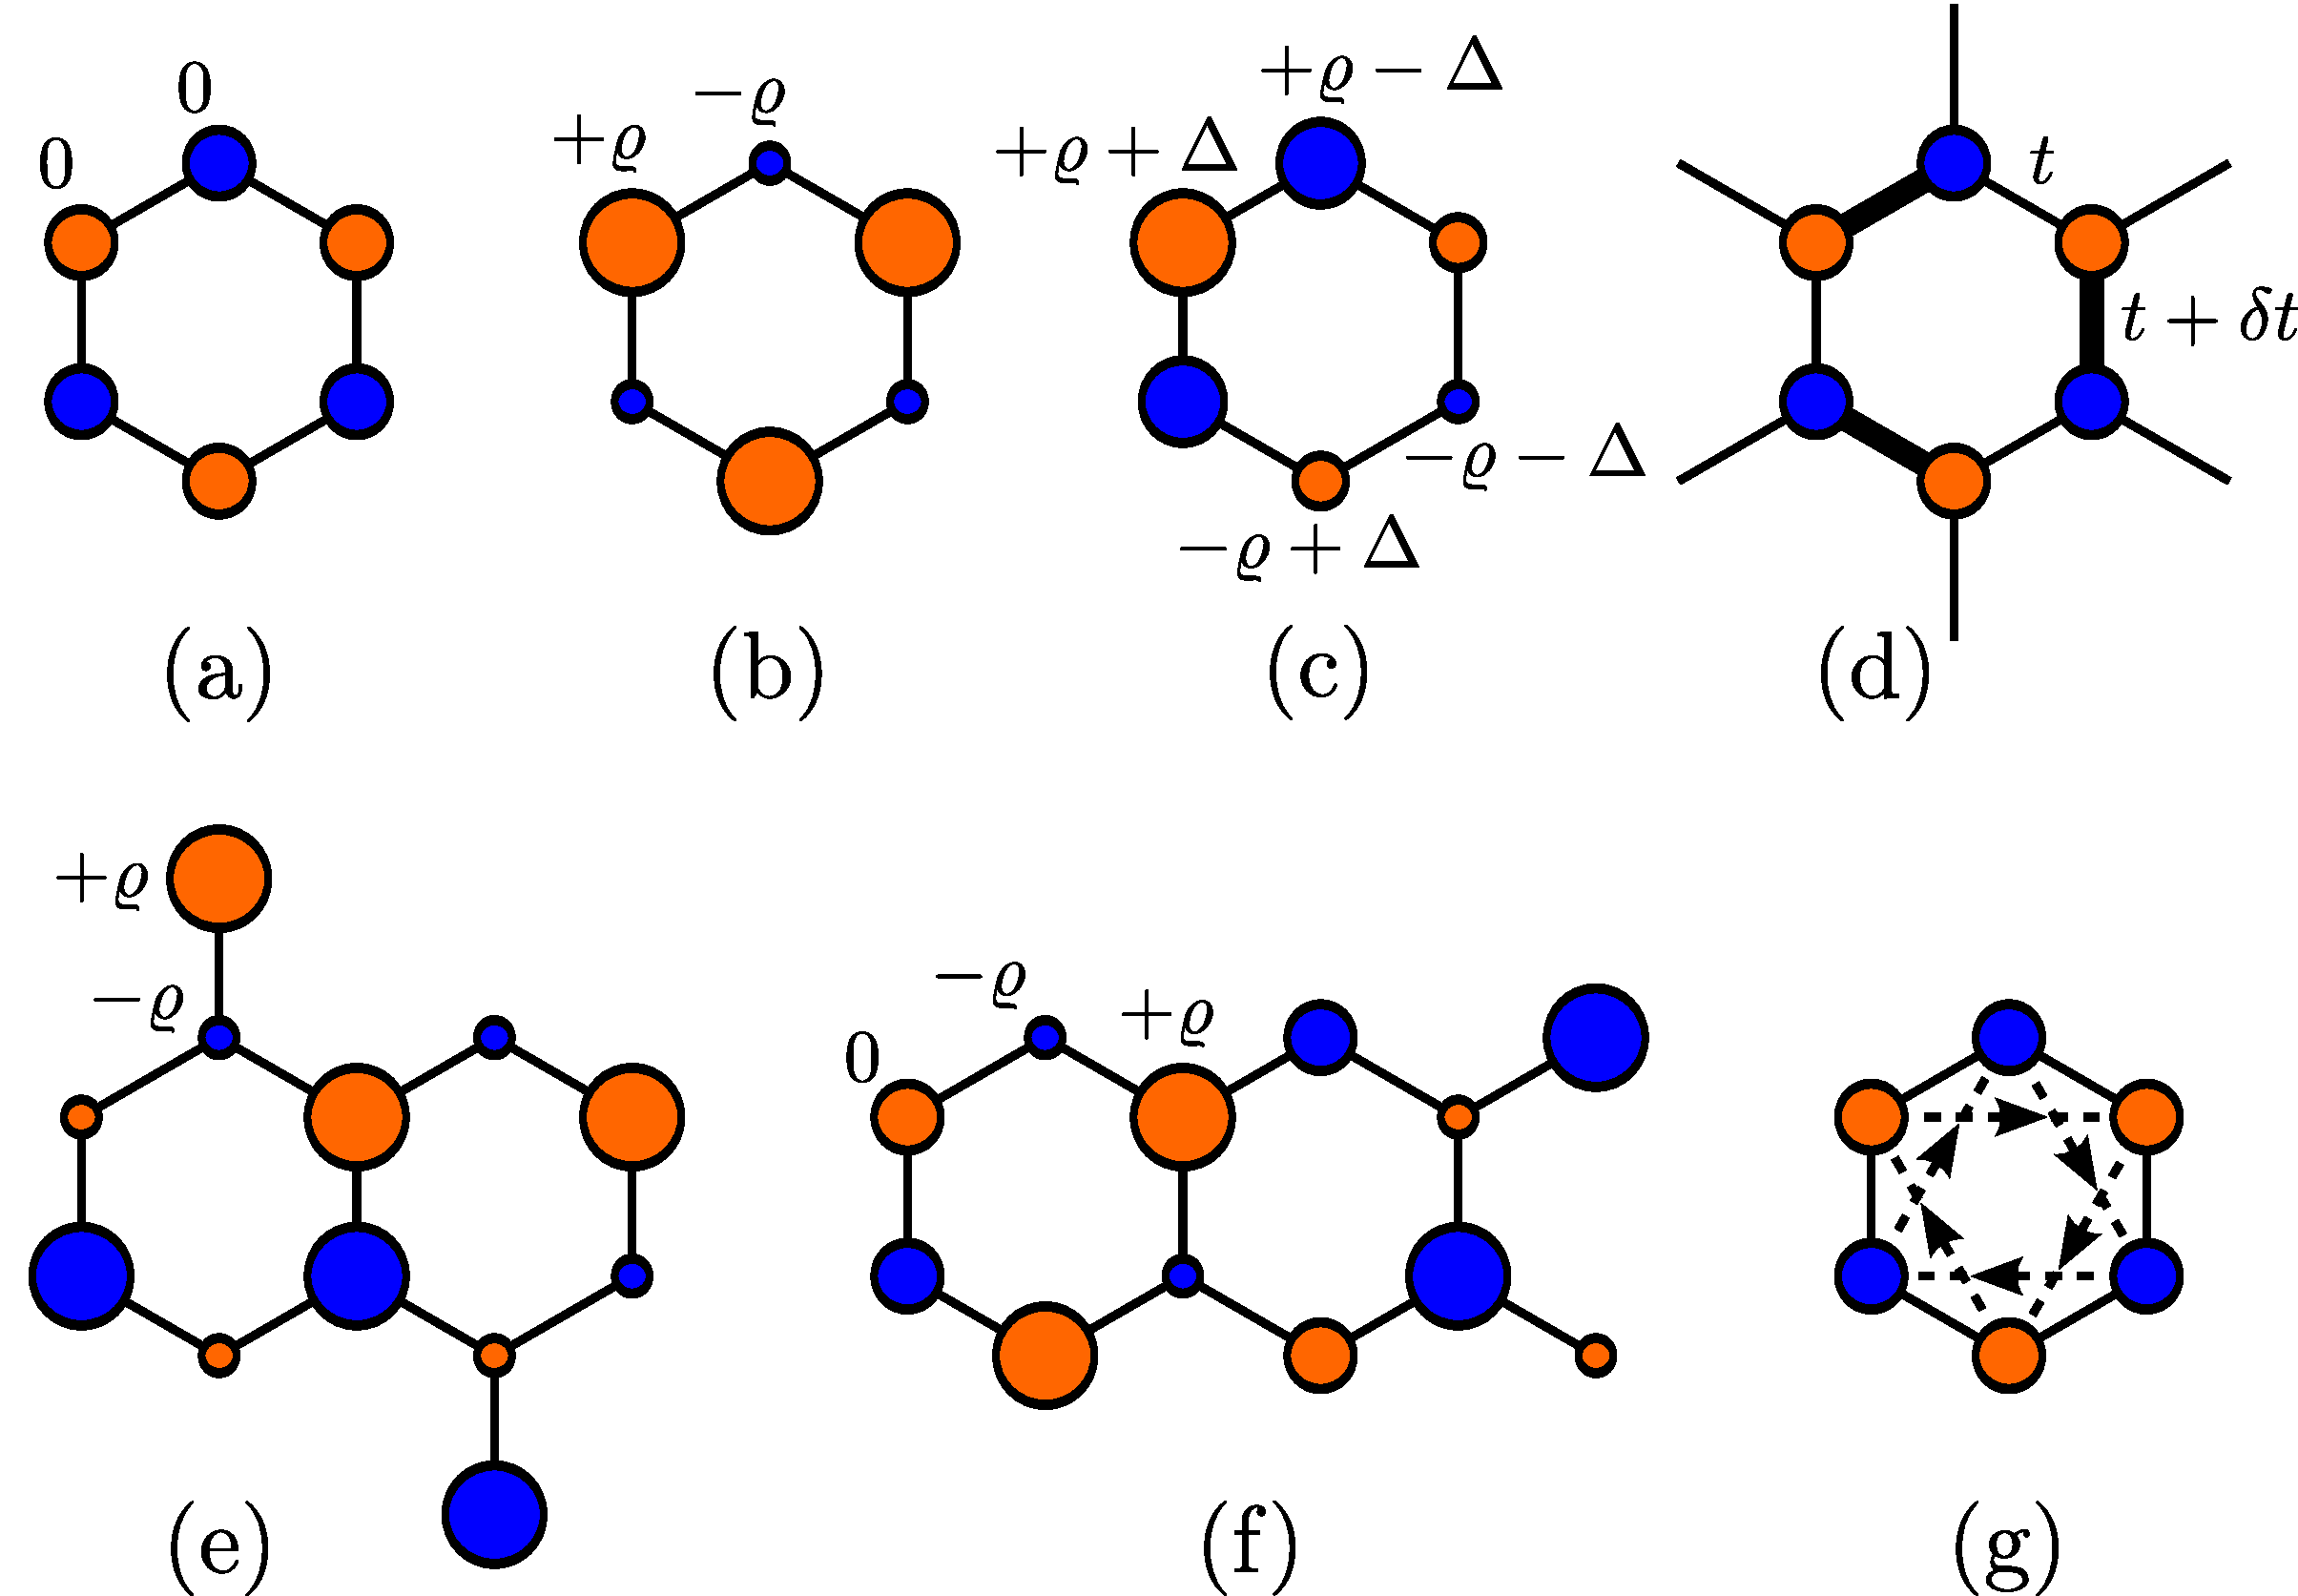
\includegraphics[width=\columnwidth]{{pdf/orders}.pdf}
 %
 \caption{Different orders allowed in the half-filled spineless Honeycomb lattice considered in this work:
 % 
 (a) Semimetal, (b) CDW I, (c) CMs, (d) Kekul\'e, (e) CDW II, (f) CDW III, (g) Haldane phase. 
 %
 Phases (a)-(d) and (g) where found within mean field theory by Refs.~\cite{Raghu,Franz,us}.
 %
The survival of the Haldane Chern insulator phase (g) was challenged within exact diagonalization in periodic boundary conditions
by Refs.~\cite{us2,Maria} but found in Ref.~\cite{Herbut} for open boundary conditions.
 %
 The existence of phase (c) was challenged with exact diagonalization by Ref.~\cite{}.
 %
 \label{fig:orders}}
 %
\end{figure}
%
This work addresses the latter problem, in particular the possibility to induce a topological state from a trivial state via strong interactions.
%
The concrete question that we consider has so far
remained controversial: the realisation of the Chern insulator phases triggered by short-range electron-electron interactions in tight binding models.
%
The Chern insulator state, first identified by Haldane~\cite{H88} in the particular case of the honeycomb lattice, is a zero field analogue of the
integer quantum Hall effect; the Hall conductivity contribution of each band is quantised in integer units of $e^2/h$ and determined by a topological invariant, the Chern number.
%
However, realising a Chern insulator in nature is not a trivial task since time-reversal must be broken but in such a way that
the resulting magnetic flux has to average to zero over the unit cell, and thus over the entire sample.
%
In a remarkable proof of principle, a set of mean field studies~\cite{Raghu,Franz,Castro} showed that the Chern insulator can 
occur from electron-electron interactions. 
%
It was shown that spiness electrons hoping in the half-filled honeycomb lattice with nearest and next-to-nearest neighbour interactions, $V_{1}$ and $V_{2}$ respectively, 
displayed a Chern insulator phase as described by Haldane.
%
This particular realization of the Chern insulator phase has complex nearest neighbour hopings (see Fig.~\ref{fig:orders}(g))
and therefore within the mean field paradigm occurs appeared in the region where $V_{2}>V_{1}$.
%
The latter condition 
was shown not to be a generic requirement; Chern insulator phases can be realized 
in mean field with only $V_{1}$ at the expense of enlarging the unit cell and doping the system.
%
In addition, analogous topological phases have been obtained in other lattices such as the square lattice~\cite{Franz}.\\

The important question that still remains to be answered is wether the interaction induced Chern state survives 
after the effect of quantum fluctuations is included.
%
The Haldane Chern insulator phase competes with more conventional but also interesting orders, 
that can jeopardise its emergence and are depicted schematically in Fig.~\ref{fig:orders}.
%
On the one hand, in the $V_{1} \gg V_{2}$ limit, a charge ordered state depicted in Fig.~\ref{fig:orders}(b) is expected, 
where the A and B sub lattices are populated differently.
%
Being connected to the classically ground state at $V_{1}/t \to \infty$ this state (CDW-I) has been found to be very robust both in mean field an exact diagonalization.
%
For $V_{2}\gg V_{1}$ on the other hand it was shown~\cite{us} in mean field that the phase space originally attributed to the Haldane Chern insulator 
was severely reduced by the presence of a sublattice charge modulated state (or CMs) Fig.~\ref{fig:orders}(c).
%
The CMs phase was corroborated to survive quantum fluctuations in exact diagonalization \cite{us} and within \noteAG{Herbuts technique}.
%
However, its existence was questioned by Ref.~\cite{} where it was argued that a pinball liquid state -- a state where a fraction of electrons remains pinned to fixed lattice sites while the remaining fermions explore the unoccupied sites -- cannot be discarded. 
%
At intermediate $V_{1}\sim V_{2}$ a Kekul\'e bond order depicted in Fig.~\ref{fig:orders}(d), that triples the original honeycomb two atom unit cell, 
was found to be stable within mean field theory.
%
Although some hints of this bond order was found~\ref{us} In exact diagonalization, further insights are needed to corroborate its existence in the thermodynamic limit.
%
The Haldane Chern insulator phase of Fig.~\ref{fig:orders}(g), stable within mean field, was found however to be absent in exact diagonalization with periodic boundary conditions~\ref{us,dag} and \noteAG{ Daghofers technique} suggesting that quantum fluctuations indeed destabilise its emergence.
%
However, this interpretation was challenged by Ref.~\ref{Herbut} that observed hints of this phase with exact diagonalization with open boundary conditions and  \noteAG{Herbuts technique}.\\

%
The contradictory numerical evidence regarding the existence of the Chern insulator phase in particular, and other competing phases in general, claims for an alternative study
that includes quantum fluctuations but suffers in the least possible way finite size effects.
%
In this work we revisit the controversies left unsolved by previous works using the infinite density matrix renormalization group method (iDMRG). 
%
This method...\noteAG{say something}.
\\
%
Our main findings are the following. 
%
First we show compelling numerical evidence that supports the absence of the Chern insulator state in a wide region of $\left\lbrace V_{1},V_{2}\right\rbrace$ phase space.
%
Second, we provide evidence for the existence and stability of the CMs state, not only from iDMRG method numerics but also from
from robust semiclassical arguments.
%
Third, we find two new phases not reported previously neither within mean field or exact diagonalization results and give a semiclassical argument for one 
of these to occur.



\section{\label{sec:modandmeth}Model and Method}
%
We investigate a system of spinless electrons hoping on a honeycomb lattice with real nearest neighbor hopping $t$ interacting via nearest and next to nearest neighbor interactions 
$\left\lbrace V_{1},V_{2}\right\rbrace$ respectively. 
%
The Hamiltonian for this system can be written as
 %
% \begin{eqnarray}
% \nonumber
%
% H&:=&-t\sum_{\left\langle i,j\right\rangle ,s,s'}(c^{\dagger}_{i,s}c_{j,s'}+h.c.)\\
% %
% \;&+&
% V_{1}\sum_{\left\langle i,j\right\rangle ,s }n_{i,s}n_{j,\bar{s}}+
% %
% V_{2}\sum_{\left\langle \left\langle i,j\right\rangle \right\rangle ,s }n_{i,s}n_{j,s}.
%
% \end{eqnarray}
\begin{equation}
 H:=-t\sum_{\left\langle i,j\right\rangle}(c^{\dagger}_{i}c^{\vphantom{\dagger}}_{j}+ \mathrm{h.c.})+
V_{1}\sum_{\left\langle i,j\right\rangle }n_{i}n_{j}+
V_{2}\sum_{\left\langle \left\langle i,j\right\rangle \right\rangle }n_{i}n_{j}.
\label{eq:H}
\end{equation}
%
where $c_{i}^{\vphantom{\dagger}}$ $(c^{\dagger}_{i})$  annihilates (creates) an electron at the $i$-th site of the honeycomb lattice.
% in sublattice $s=A,B$ and $s\neq\bar{s}$. 
%
% Each of the two triangular sublattices A and B is spanned by the basis vectors
% $\bs{a}_{1}=\bs{\delta}_{2}-\bs{\delta}_{3}$ and 
% $\bs{a}_{2}=\bs{\delta}_{3}-\bs{\delta}_{1}$ defined through the three nearest neighbors $\bs{\delta}_{1}=a(0,-1)$,  
% $\bs{\delta}_{2}=a(\sqrt{3}/2,1/2)$ and $\bs{\delta}_{3}=a(-\sqrt{3}/2,+1/2)$ as shown in Fig.~\ref{fig:Defs}.\\
%

In order to find the ground state of the system in the $\left\lbrace V_{1},V_{2}\right\rbrace$ phase space
we use the infinite density matrix renormalzation group algorithm (iDMRG) \cite{M08,W92,KZM13}. Traditionally a method for finding the ground state of one-dimensional systems, it has been proven successful in numerous examples of two-dimensional systems in which the size in one dimension is kept finite \cite{papers}. 

A generic quantum state on a chain of length $N$ can be written as a matrix product state (MPS) in the following form
\begin{equation}
 \ket{\psi} = \sum_{j_1, \ldots, j_N} A^{1 \left[j_1\right]} A^{2 \left[j_2\right]} \ldots A^{N \left[j_N\right]} \ket{j_1, \ldots, j_N}
\end{equation}
where $A^{n \left[j_n\right]}$ is a $\chi_{n-1} \times \chi_n$ matrix, $\ket{j_n}$ are the local basis states on site $n$ and the $\chi_n$ are called bond dimensions. On an infinite chain, the state is represented by an infinite matrix product state (iMPS), that is, an infinite number of matrices. However, if the chain is translationally invariant, the matrices repeat themselves after translating the system by the length of one unit cell. Hence, specifying the set of matrices in one unit cell already completely represents the state. For an arbitrary state on an infinite chain, the bond dimensions are generically also infinite. Nevertheless, the ground state of gapped systems can be approximated to any required precision by matrices of a finite bond dimension that grows with the entanglement between two semi-infinite halves of the system. \noteJM{Scaling and references}

We investigate the model on an infinite cylinder geometry and choose a unit cell of three rings of $L=12$ sites wrapping around the cylinder as depicted in Fig.~\ref{fig:Defs}. This size secures that all the possible orders that occur in the range of our study are commensurate with the iMPS unit cell. Another reason to choose this size originates from the single particle momentum discretization in the $y$-direction around the cylinder. In the non-interacting case, the model forms a Dirac semimetal with the Fermi surface consisting of the $K$ and $K^{\prime}$ points which possess momenta $k_y=k_y^{\prime} = 2\pi / 3$. Only if these two points are allowed momenta of the investigated system, the low energy physics can be captured correctly. This means that from the feasible system sizes only $L=6$ and $12$ are well suited for our purposes whereas $L=8$ and $10$ do not include the momenta of the $K$ and $K^{\prime}$ points.
%



\noteAG{we might want to define the entanglement spectrum here also if we ever use it}\\
\noteAG{Define correlation length as well}
%

\begin{figure}
 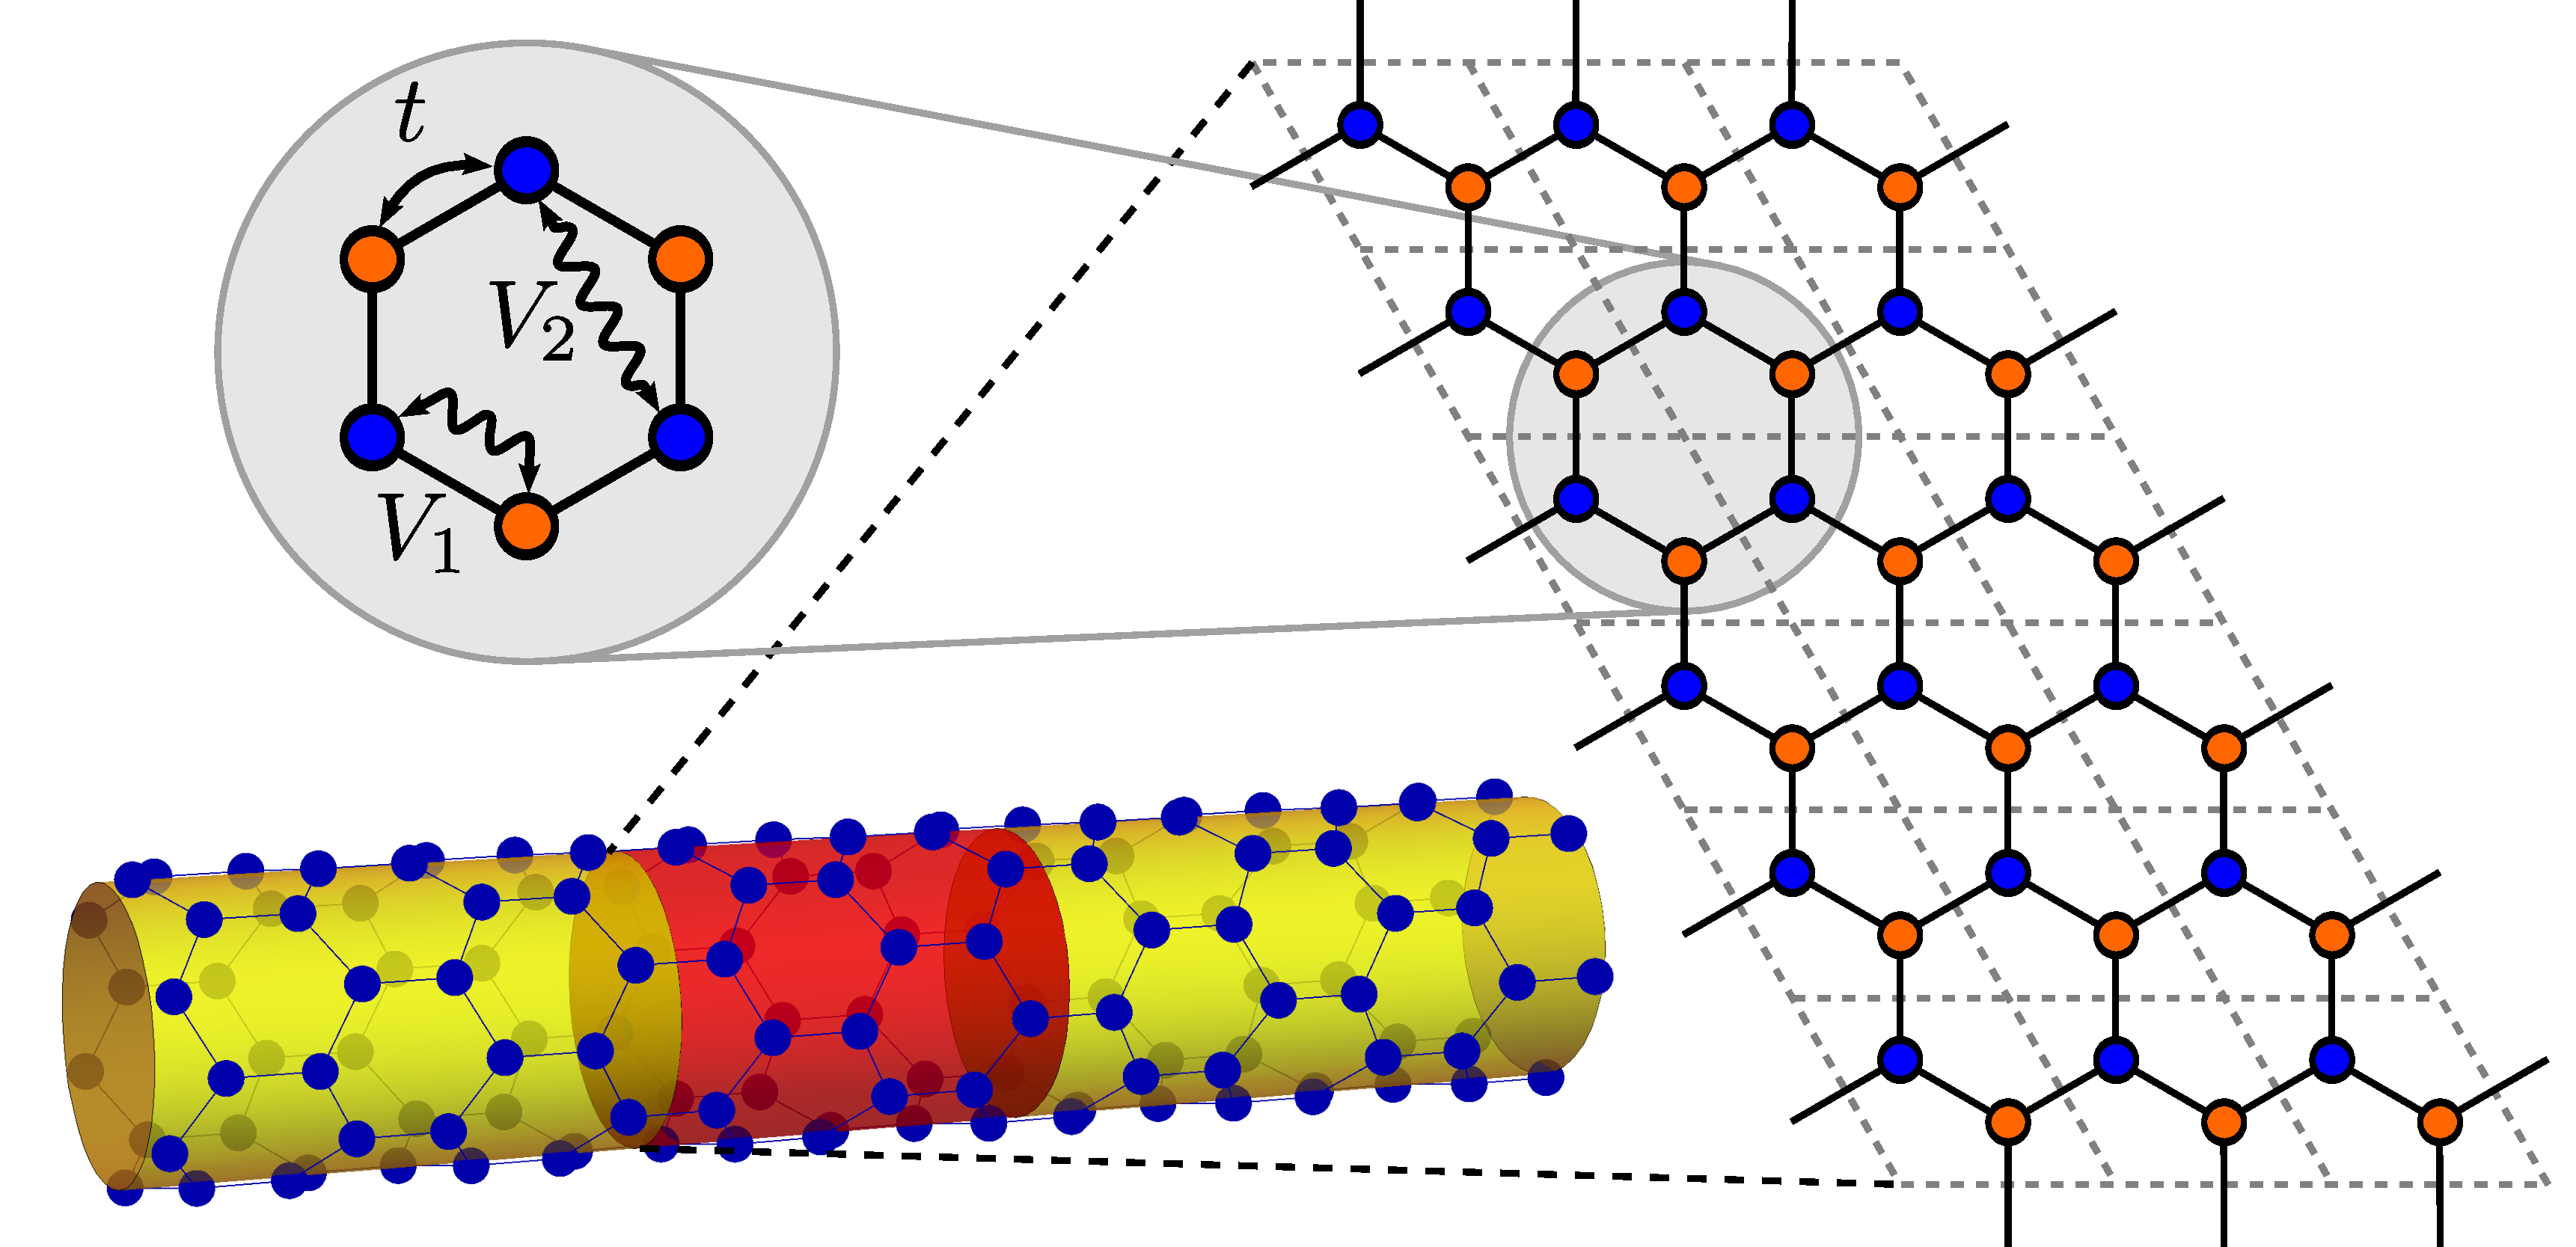
\includegraphics[width=\columnwidth]{pdf/unit_cell.pdf}
 \caption{Unit cell used in the iDMRG calculations. It consists of $3 \times 6$ lattice unit cells which yields a cylinder with a circumference of 12 sites. The hoppings and and interactions of Hamiltonian \eqref{eq:H} are shown in the gray inset.  \label{fig:Defs}}
\end{figure}
%% 
\section{Phase diagram}
%
We have used the iDMRG method presented in the previous section
to find the groundstate of the half-filled graphene lattice in the presence of 
$\left\lbrace V_{1},V_{2}\right\rbrace$ interactions.
%
Our results are summarised in the phase diagram presented in Fig.~\ref{fig:phase diagram}.

\begin{figure*}
 
\includegraphics[width=\textwidth]{pdf/phase_diagram_ext.pdf}
 \caption{Left: Phase diagram obtained with iDMRG calculations on an infinte cylinder of circumference $L=12$. Right: Density patterns in the different phases. The area of the blue circles is proportional to the particle number expectation value on the respective site. The unit cells are depicted by the red polygons. (a) Charge modulated (CMs) phase with $V_1 = 0.8, V_2 = 3.2 $, (b) Charge density wave II (CDW II) with $V_1 = 5.6, V_2 = 3.2$,  (c) Charge density wave III (CDW III) with $V_1 = 9.2, V_2 = 2.5$, (d) Charge density wave I (CDW I) with $V_1 = 4.0, V_2 = 0.4 $. Figures (e) and (f) show the density and hopping amplitude patterns of the Kekul\'e phase. The state shows a uniform density but the hopping amplitudes break translational symmetry and form a six site unit cell. \label{fig:phase diagram}}
\end{figure*}

%
As a function of $\left\lbrace V_{1},V_{2}\right\rbrace$ we find six different phases and none of them correspond to the Haldane Chern insulator.
%
In what follows we describe their corresponding charge and bond ordering patterns and analyse the different phase transitions that occur between them.
%


%
\subsection{Semimetal phase (SM)}
%
We start by discussing the semimetal phase, labelled SM in the phase diagram shown in Fig.~\ref{phase diagram}.
%
This phase is continuously connected to the gapless non-interacting state $V_{1}=V_{2}=0$; 
it is a uniform renormalization of the hopping strength $t$ by interactions.
%
Therefore we identify this state as a single particle gapless phase that lacks both charge and bond order and is described by a low energy theory in terms of two massless Dirac fermions.
%
We note that in such low energy picture and within the renormalisation group approach the stability of the semimetal phase in the region $\left\lbrace V_{1},V_{2}\right\rbrace < t$ is expected.
%
Short range interactions are irrelevant~\cite{Shankar?} and therefore they can only drive a transition to an ordered state when they have a magnitude comparable to the nearest neighbour hopping strength $t$.
%
Accordingly we find that the semimetal is stable within this region of phase space.


Within the iDMRG algorithm we have characterised the semimetal phase in three distinct ways.
%
Firstly we compute the charge and bond ground state expectation values.
%
On the one hand, at each site the charge expectation value is defined by 
%
\begin{eqnarray}
\label{eq:charge}
n_{i,s}=\left\langle c^{\dagger}_{i,s}c_{i,s}\right\rangle,  
\end{eqnarray}
%
where $s=A,B$ is the sublattice index.
%
To numerical accuracy we find that $n_{i,A}=n_{i,B}=1/2$, indicating that this phase is not charge ordered.
%

The bond ground state expectation value on the other hand is defined as
%
\begin{eqnarray}
\label{eq:bond}
t^{s,s'}_{i,j}=\left\langle c^{\dagger}_{i,s}c_{j,s'}\right\rangle,  
\end{eqnarray}
%
For $i,j$ being nearest neighbours we find a small ($10^{-?}$ \noteAG{number needed}) asymmetry
between bonds pointing along and around the cylinder axis.
%
Such asymmetry should vanish in a perfect semimetalic phase and indeed it is severely reduced as the bond dimension $\chi$ is increased.
% 
This suggests that the explanation for the asymmetry is indeed the cylinder geometry implemented in iDMRG, that artificially differentiates bonds in its two perpendicular directions.
%

%
Moreover, we note that the semimetal phase is a critical state and thus in principle requires an infinite $\chi$ to represent the state.
%
This leads us to the second approach to characterise the semimetal phase that makes use of the its criticality.
%
For a critical phase the entanglement entropy is expected to show a logarithmic growth with the correlation length.
\noteAG{eqn needed}
%
The proportionality constant $c/3$ defines the central charge of the theory $c$. 
%
The semimetal has two Dirac cones and therefore it is expected that $c=2$. 
%
In the appendix...
\noteAG{This last paragraph can be removed if we don't need it}

%
Lastly we find that the low energy structure of the many-body 
entanglement spectrum of this phase exactly coincides with that of the parent non-interacting critical state.\\ 
%

%
We note finally that this state extends beyond 

\subsection{Charge density wave (CDW)}
%
The second state we identify is the charge density wave state, labelled CDW in the phase diagram of Fig.~\ref{}.
%
This state has a two site unit cell that is characterised by a finite order parameter
%
\begin{equation}
\label{eq:CDW}
%
M=\left\langle n_{A} \right\rangle-\left\langle n_{B}\right\rangle
%
\end{equation}
%
where $n_{A}$ and $n_{B}$ are the density of electrons in the $A$ and $B$ sublattice sites of the two site unit cell respectively.
%
We find that the magnitude of $M$ increases with $V_{1}$ and to numerical accuracy this phase has no appreciable bond order.\\
%

For large $V_{1}\gg t$ such a state is a natural instability since the energy is minimised by a charge imbalance between the two sub lattices.
%
Indeed, it has been found in a mean field approximation~\cite{RQHZ08,WF10,GCCdJVV13}, exact diagnoalization~\cite{GGNVC13,DH14,DCH14}, and quantum Monte Carlo simulations
\cite{WCT14}.
%


\subsection{Sub-lattice charge modulated phase (CMs)}
%
For large $V_{2}\ll t$ the ground state is classically degenerate. 
%
Within mean field it was shown that as long $V_{2}>V_{1}$
the system chose a charge ordered pattern with charge modulation over different sub lattices and termed CMs phase~\cite{CMs}.
%
Such order, schematically shown in Fig.~\ref{fig:orders}(c), has a six site unit cell, and minimises the large cost
attributed to $V_{2}$ by reversing two nearest neighbour dimers at the expense of paying the small energetic cost
determined by $V_{1}$.
%
Within in exact diagonalization two studies has shown that the CMs state survives quantum fluctuations 
but its nature was challenged in Ref.~\onlinecite{daghofer} suggesting that a pinball like state cannot be ruled out.\\

With the iDMRG method (see Fig.~\ref{s}) we find that directly above the semimetallic phase the CMs occurs with the right type of order.
%
The calculated charge pattern obtained from \eqref{eq:charge} is shown in Fig.~\ref{} panel, which resembles the expected
CMs pattern.
%
The six-site unit cell is depicted as a red hexagon for clarity. 
%
Such a state also presents bond ordering associated to the charge patterns.

% 
Moreover, we now show that the CMs state is expected from a semi-classical analysis as well.
%
For instance, for a given cluster, it is possible to find the number and energy of all the degenerate classical states, assuming $V_{2}\gg t$.
%
Within this approach, the hopping can be introduced as a perturbation $t$ to find how the degeneracy is lifted.
\noteAG{Maybe Fernando can rewrite this part better...} \noteFdJ{Test comment}


\subsection{Kekul\'{e} bond order}
%
The next phase we identify is the Kekul\'{e}
bond order.
%
Like the CMs, it has a six site unit cell depicted schematically in Fig.~\ref{}
and uniform charge order.
%
In mean field the state arises close to the $V_{1}\eqsim V_{2}$.
%
Although in exact diagonalization hints of this state are also observed,
the evidence supporting its occurrence is far from conclusive.



\subsection{Charge density wave - II}
%
All phases that we have described so far don't differ
from those predicted by mean field and exact diagonalization.
%
We have identified
%
\subsection{Charge density wave - III}
%



\section{Phase transitons}
%
A crucial advantage of the iDMRG method is that, unlike finite
size methods such as exact diagonalization it can characterize the order of phase transitions.
%
In order to unravel the character of the phase transitions between
the phases described above we now study two quantities that are sensitive
to a phase change, the entanglement entropy $S$ and the correlation length $\xi$.
%
In Fig.~\ref{}  and Fig.~\ref{} we show how these quantities change along
the horizontal and vertical cuts depicted in Fig.~\ref{fig:phase diagram} respectively.
%

\subsection{Cut A: SM--CDW-I}

The first horizontal cut, labelled A addresses the character of the phase transition between the semi-metallic
phase and the simplest charge density wave (CDW-I) by fixing $V_{2}=0$.
%
This phase transition has been previously addressed with the quantum Monte-Carlo method~\ref{WCT14} 
and was determined to be of second order character.
%
The transition point with divergent correlation length was determined to be at $V_{1}=$ via finite size scaling.
\noteAG{need number and polishing, Johannes?}
%
In Fig.~\ref{fig:cut_V2_0} we show the correlation length as a function of $V_{1}$ 
for different values of the bond dimension $\chi$ and cylinder with $L=12$ circumference.
\begin{figure}
 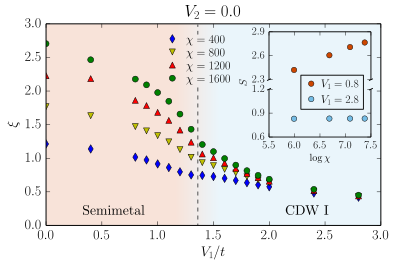
\includegraphics[width=\columnwidth]{{pdf/plot_cut_V2_0}.pdf}
 \label{fig:cut_V2_0}
 \caption{Correlation length at $V_2=0$.  \noteAG{could it be useful to show the order parameter M
 as a function of $V_{1}$ in the same plot (using the right vertical axis?). It might get to crowded)}}
\end{figure}
% 
%
Firstly, for $V_{1}\leq 1.5t$ we observe that the correlation length diverges as the bond
dimension of the MPS is increased.
%
This behaviour is expected for a critical state such as the semimetal phase;  
the logarithmic divergence of entanglement of a metallic state requires an MPS with $\chi\to\infty$.
%
For $V_{1}\geq 1.5t$ the correlation length drops significantly and has no longer a significant 
dependence on $\chi$.
%
This is characteristic of a gapped phase such as the charge density wave.
%
The crossover is smooth, signalling a second order phase transition, in agreement with 
quantum Monte Carlo studies.
%
With iDMRG it is however not possible to pin point the exact value of $V_{1}$ 
where the transition happens via finite size scaling due to the few cylinder sizes 
we have available, as discussed in section \ref{sec:modandmeth}.
%
However, from Fig.~\ref{} it is however possible to define a crossover region $1.4 \leq V_{1}\geq 2$,
consistent with the quantum Monte Carlo data, where the transition occurs.

\subsection{Cut B: SM--CMs}
%
The cut at $V_{1}=0.4$, labelled cut B in Fig.~\ref{fig:phase diagram}, 
probes the transition between the semimetal phase and the CMs phases.
%
In Fig.~\ref{fig:cut_V1_0.4} we present the entanglement entropy $S$ as a function of $V_{2}$
, the interaction that drives the phase transition.

\begin{figure}
 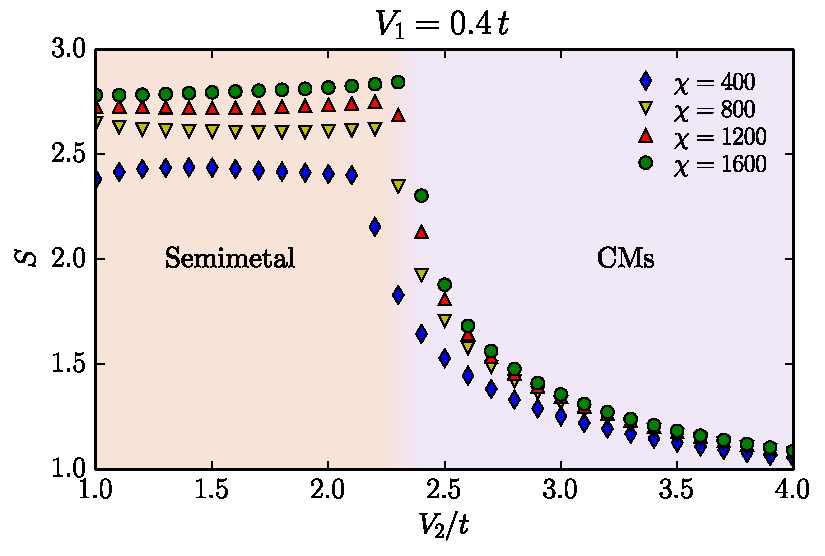
\includegraphics[width=\columnwidth]{{pdf/plot_cut_V1_0.4}.pdf}
 \caption{Entanglement entropy at $V_1=0.4$. \label{fig:cut_V1_0.4}}
\end{figure}
%
As expected from the previous analysis the entanglement entropy of 
the semimetal phase depends strongly on the MPS bond dimension $\chi$.
%
At $V_{2}\approx $ \noteAG{need value} we observe a sharp transition
to a decaying entanglement entropy that does not depend strongly on $\chi$
as $V_{2}$ is increased from the transtion.
%
This evidence is suggestive of a first order phase transition between
the semimetal and CMs phases.
%
The correlation length (not shown) also shows a discontinuity but not
as pronounced as the entanglement entropy.
%
\noteAG{Do we have an idea of why $S$ is better than $\xi$ sometimes to show phase transitions?}

\subsection{Cut C: CMs--CDW-II}

In cut C we fix $V_{2}=3.6$ and study the phase transition between
the CMs and the CDW-II phases.
%
The entanglement entropy is shown in Fig.~\ref{fig:cut_V2_3.6} 
as a function of $V_{1}$.
\begin{figure}
 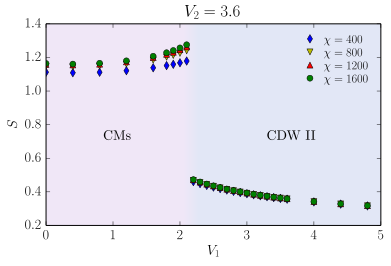
\includegraphics[width=\columnwidth]{{pdf/plot_cut_V2_3.6}.pdf}
 \caption{Entanglement entropy at $V_2=3.6$. \label{fig:cut_V2_3.6}}
\end{figure}
% 
%
This quantity shows a clear jump at $V_{2}\approx$ signalling a direct first order
phase transition between these two phases.
%
\noteAG{Is this expected semi-classically somehow?}

\subsection{Cut D: CDW-I--Kekul\'{e}--SM--CDW-II}

\begin{figure}
 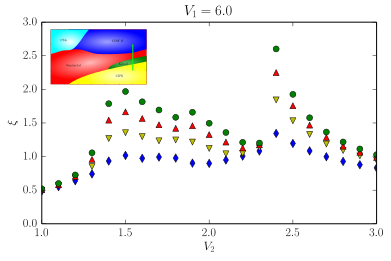
\includegraphics[width=\columnwidth]{{pdf/plot_cut_V1_6}.pdf}
 \caption{Correlation length at $V_1=6$. \label{fig:cut_V1_6}}
\end{figure}


\subsection{Cut E: SM--CDW-III}





% 




%
\section{Discussion and Conclusions}
%



No CI phase\\
%
Two new phases not seen before\\
%
What determines if $S$ or $\xi$ gives better signatures of phase transitions. \\
%
Expect the same to happen in square lattice.

\section{Acknowledgements}

We thank A. Läuchli for discussions and sharing results prior to publication.

\bibliography{CI_iDMRG.bib}


\end{document}